\chapter{Software}
\label{app:fastpli}

% \section{fastpli}
% \lstinputlisting[language=python, caption=src/fastpli/\_\_init\_\_.py]{code/src/fastpli/__init__.py}
% \section{fastpli/analysis}
% %\lstinputlisting[language=python, caption=src/fastpli/analysis/\_ROFL\_with\_jacobi.py]{code/src/fastpli/analysis/_ROFL_with_jacobi.py}
% \lstinputlisting[language=python, caption=src/fastpli/analysis/\_\_init\_\_.py]{code/src/fastpli/analysis/__init__.py}
% \lstinputlisting[language=python, caption=src/fastpli/analysis/affine\_transformation.py]{code/src/fastpli/analysis/affine_transformation.py}
% \lstinputlisting[language=python, caption=src/fastpli/analysis/epa.py]{code/src/fastpli/analysis/epa.py}
% \lstinputlisting[language=python, caption=src/fastpli/analysis/images.py]{code/src/fastpli/analysis/images.py}
% \lstinputlisting[language=python, caption=src/fastpli/analysis/orientation.py]{code/src/fastpli/analysis/orientation.py}
% \lstinputlisting[language=python, caption=src/fastpli/analysis/rofl.py]{code/src/fastpli/analysis/rofl.py}
% \section{fastpli/io}
% \lstinputlisting[language=python, caption=src/fastpli/io/\_\_init\_\_.py]{code/src/fastpli/io/__init__.py}
% \lstinputlisting[language=python, caption=src/fastpli/io/fiber.py]{code/src/fastpli/io/fiber.py}
% \lstinputlisting[language=python, caption=src/fastpli/io/label\_converter.py]{code/src/fastpli/io/label_converter.py}
% \section{fastpli/model}
% \lstinputlisting[language=python, caption=src/fastpli/model/\_\_init\_\_.py]{code/src/fastpli/model/__init__.py}
% \lstinputlisting[language=python, caption=src/fastpli/model/\_visualizer.py]{code/src/fastpli/model/_visualizer.py}
% \section{fastpli/model/sandbox}
% \lstinputlisting[language=python, caption=src/fastpli/model/sandbox/\_\_init\_\_.py]{code/src/fastpli/model/sandbox/__init__.py}
% \lstinputlisting[language=python, caption=src/fastpli/model/sandbox/build.py]{code/src/fastpli/model/sandbox/build.py}
% \lstinputlisting[language=python, caption=src/fastpli/model/sandbox/seeds.py]{code/src/fastpli/model/sandbox/seeds.py}
% \section{fastpli/model/solver}
% \lstinputlisting[language=python, caption=src/fastpli/model/solver/\_\_init\_\_.py]{code/src/fastpli/model/solver/__init__.py}
% \lstinputlisting[language=python, caption=src/fastpli/model/solver/\_solver.py]{code/src/fastpli/model/solver/_solver.py}
% \section{fastpli/objects}
% \lstinputlisting[language=python, caption=src/fastpli/objects/\_\_init\_\_.py]{code/src/fastpli/objects/__init__.py}
% \lstinputlisting[language=python, caption=src/fastpli/objects/fiber.py]{code/src/fastpli/objects/fiber.py}
% \lstinputlisting[language=python, caption=src/fastpli/objects/fiber\_bundle.py]{code/src/fastpli/objects/fiber_bundle.py}
% \lstinputlisting[language=python, caption=src/fastpli/objects/fiber\_bundles.py]{code/src/fastpli/objects/fiber_bundles.py}
% \section{fastpli/simulation}
% \lstinputlisting[language=python, caption=src/fastpli/simulation/\_\_init\_\_.py]{code/src/fastpli/simulation/__init__.py}
% \lstinputlisting[language=python, caption=src/fastpli/simulation/\_simpli.py]{code/src/fastpli/simulation/_simpli.py}
% \lstinputlisting[language=python, caption=src/fastpli/simulation/optic.py]{code/src/fastpli/simulation/optic.py}
% \section{fastpli/tools}
% \lstinputlisting[language=python, caption=src/fastpli/tools/\_\_init\_\_.py]{code/src/fastpli/tools/__init__.py}
% \lstinputlisting[language=python, caption=src/fastpli/tools/helper.py]{code/src/fastpli/tools/helper.py}
% \lstinputlisting[language=python, caption=src/fastpli/tools/rotation.py]{code/src/fastpli/tools/rotation.py}
% \section{include}
% \section{model}
% \section{model/solver}
% \lstinputlisting[language=c++, caption=src/model/solver/cone\_class.cpp]{code/src/model/solver/cone_class.cpp}
% \lstinputlisting[language=c++, caption=src/model/solver/fiber\_class.cpp]{code/src/model/solver/fiber_class.cpp}
% \lstinputlisting[language=c++, caption=src/model/solver/oct\_tree.cpp]{code/src/model/solver/oct_tree.cpp}
% \lstinputlisting[language=c++, caption=src/model/solver/scene.cpp]{code/src/model/solver/scene.cpp}
% \lstinputlisting[language=c++, caption=src/model/solver/world.cpp]{code/src/model/solver/world.cpp}
% \section{model/solver/bindings}
% \lstinputlisting[language=c++, caption=src/model/solver/bindings/solver\_module.cpp]{code/src/model/solver/bindings/solver_module.cpp}
% \section{objects}
% \lstinputlisting[language=c++, caption=src/objects/cell.cpp]{code/src/objects/cell.cpp}
% \lstinputlisting[language=c++, caption=src/objects/fiber.cpp]{code/src/objects/fiber.cpp}
% \section{simulation}
% \lstinputlisting[language=c++, caption=src/simulation/cell\_population.cpp]{code/src/simulation/cell_population.cpp}
% \lstinputlisting[language=c++, caption=src/simulation/fiber\_bundle.cpp]{code/src/simulation/fiber_bundle.cpp}
% \lstinputlisting[language=c++, caption=src/simulation/generator.cpp]{code/src/simulation/generator.cpp}
% \lstinputlisting[language=c++, caption=src/simulation/my\_mpi.cpp]{code/src/simulation/my_mpi.cpp}
% \lstinputlisting[language=c++, caption=src/simulation/simulator.cpp]{code/src/simulation/simulator.cpp}
% \section{simulation/bindings}
% \lstinputlisting[language=c++, caption=src/simulation/bindings/generator\_module.cpp]{code/src/simulation/bindings/generator_module.cpp}
% \lstinputlisting[language=c++, caption=src/simulation/bindings/simulator\_module.cpp]{code/src/simulation/bindings/simulator_module.cpp}

% \chapter{Appendix B}
% % 
% \begin{figure}[!tb]
% \centering
% \resizebox{0.875\textwidth}{!}{
% \def\fiberradius{0.5}
% \inputtikz{dev/gfx/2/cube_stat.tex}}
% \caption{at fl=3 somethings wrong with the first fr value.
% Better use time, steps depends on every variable!}
% % \label{fig:}
% \end{figure}
% % 
% \begin{figure}[!tb]
% \centering
% \resizebox{0.875\textwidth}{!}{
% \def\fiberradius{1.0}
% \inputtikz{dev/gfx/2/cube_stat.tex}}
% \caption{at fl=3 somethings wrong with the first fr value.
% Better use time, steps depends on every variable!}
% % \label{fig:}
% \end{figure}
% % 
% \begin{figure}[!tb]
% \centering
% \resizebox{0.875\textwidth}{!}{
% \def\fiberradius{2.0}
% \inputtikz{dev/gfx/2/cube_stat.tex}}
% \caption{at fl=3 somethings wrong with the first fr value.
% Better use time, steps depends on every variable!}
% % \label{fig:}
% \end{figure}
% 
% \begin{figure}[!tb]
% \centering
% \resizebox{0.875\textwidth}{!}{
% \def\fiberradius{5.0}
% \inputtikz{dev/gfx/2/cube_stat.tex}}
% \caption{at fl=3 somethings wrong with the first fr value.
% Better use time, steps depends on every variable!}
% % \label{fig:}
% \end{figure}
% % 
% \begin{figure}[!tb]
% \centering
% \resizebox{0.875\textwidth}{!}{
% \def\fiberradius{10.0}
% \inputtikz{dev/gfx/2/cube_stat.tex}}
% \caption{at fl=3 somethings wrong with the first fr value.
% Better use time, steps depends on every variable!}
% % \label{fig:}
% \end{figure}
% 
% \chapter{Appendix C}
% \begin{figure}[!tb]
% \centering
% \resizebox{1.0\textwidth}{!}{
% \begin{tikzpicture}[>=latex]
% \node[inner sep=0pt] (image) at (0,0)
%     {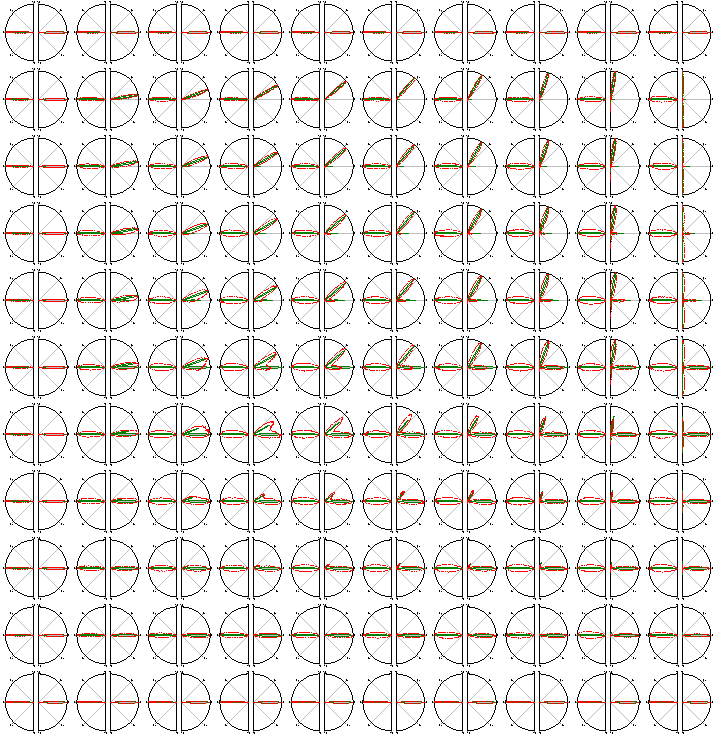
\includegraphics[width=1.0\textwidth]{gfx/model/results/model_analysis.pdf}};
% \begin{scope}[overlay]
%     \draw[->,thick] ($(image.north west)-(0.25,-0.25)$) -- ++(1,0) node [midway, above] {$\Omega$};
%     \draw[->,thick] ($(image.north west)-(0.25,-0.25)$) -- ++(0,-1) node [midway, above, rotate=90] {$\Psi$};
% \end{scope}
% \path ($(image.north west) + (-.5,.5)$) -- ($(image.north east) + (.5,.5)$);
% \end{tikzpicture}
% }
% \caption{model init vs solved}
% \label{fig:model_histogram}
% \end{figure}
% % 
% \begin{figure}[!tb]
% \centering
% \resizebox{1.0\textwidth}{!}{
% \begin{tikzpicture}[>=latex]
% \node[inner sep=0pt] (image) at (0,0)
%     {\includegraphics[width=1.0\textwidth]{gfx/model/results/histogram.pdf}};
% \begin{scope}[overlay]
%     \draw[->,thick] ($(image.north west)-(0.25,-0.25)$) -- ++(1,0) node [midway, above] {$\Omega$};
%     \draw[->,thick] ($(image.north west)-(0.25,-0.25)$) -- ++(0,-1) node [midway, above, rotate=90] {$\Psi$};
% \end{scope}
% \path ($(image.north west) + (-.5,.5)$) -- ($(image.north east) + (.5,.5)$);
% \end{tikzpicture}
% }
% \caption{Histogram cube\_2pop\_model}
% \label{fig:model_histogram}
% \end{figure}
% % 
% % 
% \begin{figure}[!tb]
% \centering
% \resizebox{1.0\textwidth}{!}{
% \begin{tikzpicture}[>=latex]
% \node[inner sep=0pt] (image) at (0,0)
%     {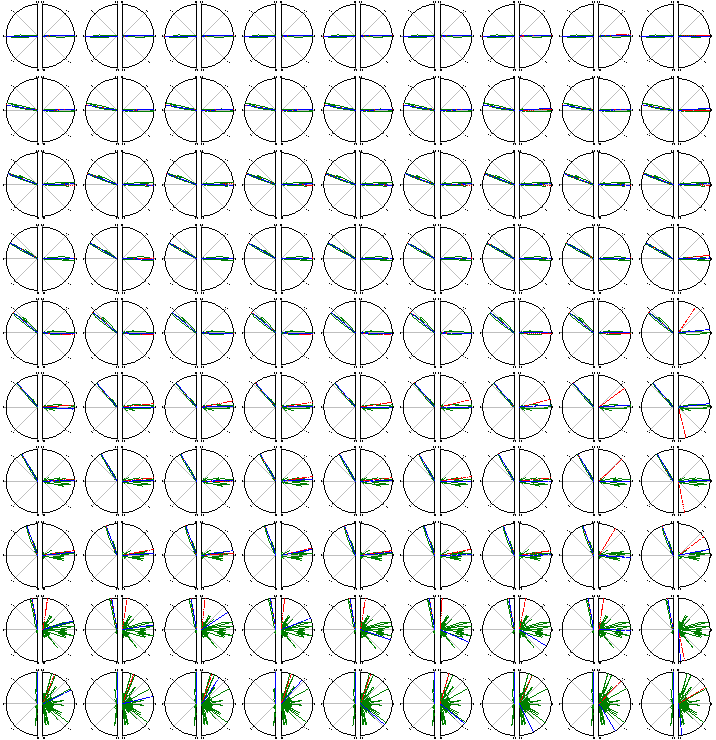
\includegraphics[width=1.0\textwidth]{gfx/model/results/voxel_size_simulation_analysis.pdf}};
% \begin{scope}[overlay]
%     \draw[->,thick] ($(image.north west)-(0.25,-0.25)$) -- ++(1,0) node [midway, above] {$voxel_size$};
%     \draw[->,thick] ($(image.north west)-(0.25,-0.25)$) -- ++(0,-1) node [midway, above, rotate=90] {$f0_inc$};
% \end{scope}
% \path ($(image.north west) + (-.5,.5)$) -- ($(image.north east) + (.5,.5)$);
% \end{tikzpicture}
% }
% \vspace{-1ex}
% \begin{center}
% \begin{tikzpicture}
%     \draw[thin] (-3.0,-0.625) rectangle (3.0,0.25);
%     \draw [green!50!black] (-2.5,0) -- (-1.5,0) node [below, midway, black] {truth};
%     \draw [red,dashed] (-0.5,0) -- (0.5,0) node [below, midway, black] {model=r};
%     \draw [blue, dash dot] (1.5,0) -- (2.5,0) node [below, midway, black] {model=p};
% \end{tikzpicture}
% \end{center}
% \caption{voxel\_size\_5\_}
% \label{fig:model_histogram}
% \end{figure}
% % 
% \begin{figure}[!tb]
% \centering
% \resizebox{1.0\textwidth}{!}{
% \begin{tikzpicture}[>=latex]
% \node[inner sep=0pt] (image) at (0,0)
%     {\includegraphics[width=1.0\textwidth]{gfx/simpli/results/simulation_analysis_spheres_LAP_p.pdf}};
% \begin{scope}[overlay]
%     \draw[->,thick] ($(image.north west)-(0.25,-0.25)$) -- ++(1,0) node [midway, above] {$\mathfrak{f}_0^\alpha$};
%     \draw[->,thick] ($(image.north west)-(0.25,-0.25)$) -- ++(0,-1) node [midway, above, rotate=90] {$\mathfrak{f}_0^\Psi$};
% \end{scope}
% \path ($(image.north west) + (-.5,.5)$) -- ($(image.north east) + (.5,.5)$);
% \end{tikzpicture}
% }
% \caption{Sphere LAP p}
% \label{fig:model_histogram}
% \end{figure}
% % 
% \begin{figure}[!tb]
% \centering
% \resizebox{1.0\textwidth}{!}{
% \begin{tikzpicture}[>=latex]
% \node[inner sep=0pt] (image) at (0,0)
%     {\includegraphics[width=1.0\textwidth]{gfx/simpli/results/simulation_analysis_spheres_LAP_r.pdf}};
% \begin{scope}[overlay]
%     \draw[->,thick] (image.north west) -- ++(1,0) node [midway, above] {$\alpha_0$};
%     \draw[->,thick] (image.north west) -- ++(0,-1) node [midway, above, rotate=90] {$\Psi_0$};
% \end{scope}
% \path ($(image.north west) + (-.5,.5)$) -- ($(image.north east) + (.5,.5)$);
% \end{tikzpicture}
% }
% \caption{Sphere LAP r}
% \label{fig:model_histogram}
% \end{figure}
% % 
% \begin{figure}[!tb]
% \centering
% \resizebox{1.0\textwidth}{!}{
% \begin{tikzpicture}[>=latex]
% \node[inner sep=0pt] (image) at (0,0)
%     {\includegraphics[width=1.0\textwidth]{gfx/simpli/results/simulation_analysis_spheres_PM_p.pdf}};
% \begin{scope}[overlay]
%     \draw[->,thick] ($(image.north west)-(0.25,-0.25)$) -- ++(1,0) node [midway, above] {$f_0$};
%     \draw[->,thick] ($(image.north west)-(0.25,-0.25)$) -- ++(0,-1) node [midway, above, rotate=90] {$\Psi$};
% \end{scope}
% \path ($(image.north west) + (-.5,.5)$) -- ($(image.north east) + (.5,.5)$);
% \end{tikzpicture}
% }
% \caption{Sphere PM p}
% \label{fig:model_histogram}
% \end{figure}
% % 
% \begin{figure}[!tb]
% \centering
% \resizebox{1.0\textwidth}{!}{
% \begin{tikzpicture}[>=latex]
% \node[inner sep=0pt] (image) at (0,0)
%     {\includegraphics[width=1.0\textwidth]{gfx/simpli/results/simulation_analysis_spheres_PM_r.pdf}};
% \begin{scope}[overlay]
%     \draw[->,thick] ($(image.north west)-(0.25,-0.25)$) -- ++(1,0) node [midway, above] {$f_0$};
%     \draw[->,thick] ($(image.north west)-(0.25,-0.25)$) -- ++(0,-1) node [midway, above, rotate=90] {$\Psi$};
% \end{scope}
% \path ($(image.north west) + (-.5,.5)$) -- ($(image.north east) + (.5,.5)$);
% \end{tikzpicture}
% }
% \caption{Sphere PM r}
% \label{fig:model_histogram}
% \end{figure}
% % 
% \begin{figure}[!t]
% \centering
% \resizebox{1.0\textwidth}{!}{
% \includegraphics[width=\textwidth, page=2]{dev/rc1/cube_2pop_orientation_hist2d_output_cube_2pop_135_rc1.pdf}
% }
% \caption[Model orientation histograms]{density distribution of fiber segment orientation in initial and resulting models for $\fiberRadius = \SI{1}{\micro\meter}$. \itodo{fit ESAG} \ITODO{these are only resulting models!}}
% \label{fig:modelOrientation}
% \end{figure}
% % 
% % 
% 
\chapter{Model analysis}
\label{app:modelAnalysis}
% 
\begin{figure}[H]
    \centering
    \includegraphics[width=1\textwidth]{dev/rc1/mpara/pre_stats_box_plot_volume_output_parameter_statistic_rc1.pdf}
    \caption{Caption}
    \label{fig:appModelVolumeBoxPlot}
\end{figure}
% 
% % \foreach \n in {1,3,...,10}{
% % \begin{landscape}
% \begin{figure}[!t]
% \centering
% % \resizebox{\textwidth}{!}{
% \includegraphics[width=\textwidth,page=1]{dev/rc1/mpara/pre_stats_time_evolve_all_output_parameter_statistic_rc1.pdf}
% \includegraphics[width=\textwidth,page=2]{dev/rc1/mpara/pre_stats_time_evolve_all_output_parameter_statistic_rc1.pdf}
% \end{figure}
% % \end{landscape}

\begin{sidewaysfigure}[]
\centering
% \resizebox{\textwidth}{!}{
\includegraphics[width=0.475\textwidth,page=1]{dev/rc1/mpara/pre_stats_time_evolve_all_output_parameter_statistic_rc1.pdf}
\includegraphics[width=0.475\textwidth,page=2]{dev/rc1/mpara/pre_stats_time_evolve_all_output_parameter_statistic_rc1.pdf}
\label{app:pste1}
\end{sidewaysfigure}
% 
\begin{sidewaysfigure}[]
\centering
% \resizebox{\textwidth}{!}{
\includegraphics[width=0.475\textwidth,page=3]{dev/rc1/mpara/pre_stats_time_evolve_all_output_parameter_statistic_rc1.pdf}
\includegraphics[width=0.475\textwidth,page=4]{dev/rc1/mpara/pre_stats_time_evolve_all_output_parameter_statistic_rc1.pdf}
\label{app:pste2}
\end{sidewaysfigure}
% 
\begin{sidewaysfigure}[]
\centering
% \resizebox{\textwidth}{!}{
\includegraphics[width=0.475\textwidth,page=5]{dev/rc1/mpara/pre_stats_time_evolve_all_output_parameter_statistic_rc1.pdf}
\includegraphics[width=0.475\textwidth,page=6]{dev/rc1/mpara/pre_stats_time_evolve_all_output_parameter_statistic_rc1.pdf}
\label{app:pste3}
\end{sidewaysfigure}
% 
\begin{sidewaysfigure}[]
\centering
% \resizebox{\textwidth}{!}{
\includegraphics[width=0.475\textwidth,page=7]{dev/rc1/mpara/pre_stats_time_evolve_all_output_parameter_statistic_rc1.pdf}
\includegraphics[width=0.475\textwidth,page=8]{dev/rc1/mpara/pre_stats_time_evolve_all_output_parameter_statistic_rc1.pdf}
\label{app:pste4}
\end{sidewaysfigure}
% 
\begin{sidewaysfigure}[]
\centering
% \resizebox{\textwidth}{!}{
\includegraphics[width=0.475\textwidth,page=9]{dev/rc1/mpara/pre_stats_time_evolve_all_output_parameter_statistic_rc1.pdf}
\includegraphics[width=0.475\textwidth,page=10]{dev/rc1/mpara/pre_stats_time_evolve_all_output_parameter_statistic_rc1.pdf}
\label{app:pste5}
\end{sidewaysfigure}
% 
\begin{figure}
    \centering
    \includegraphics[width=\textwidth, page=2]{dev/rc1/cube_2pop_orientation_hist2d_output_cube_2pop_135_rc1.pdf}
    \caption{Caption}
    \label{fig:modelHistOrientation}
\end{figure}[]
% 
% 
\begin{figure}[!t]
\centering
\includegraphics[page=2]{dev/rc1/speed/boxplot_output_r_0.5.pkl_speedup.csv.pdf}
\caption[\code{model.Sovler} speedup]{\code{model.Sovler} speedup. The time measurements are taken after $\Delta_{\mathit{steps}}$ for the next $\SI{25}{\steps}$ for parallel $(||)$ and crossing $(\times)$ fiber configurations.}
\label{fig:solverSpeedupAll}
\end{figure}
% 
% 
% 
\chapter{Simulation}
% 
\includegraphics[width=0.95\textwidth]{dev/rc1/tissue/bf_rc1_retardation_PM_Roden.pdf}
\includegraphics[width=0.95\textwidth]{dev/rc1/tissue/bf_rc1_retardation_PM_Human.pdf}
\includegraphics[width=0.95\textwidth]{dev/rc1/tissue/bf_rc1_transmittance_PM_Roden.pdf}
\includegraphics[width=0.95\textwidth]{dev/rc1/tissue/bf_rc1_transmittance_PM_Human.pdf}
% 
\begin{figure}[!p]%p
% 2_simulation/0_parameter/fiber_radii.py
\centering
\includegraphics[width=\textwidth, page=1]{dev/rc1/voxel_size/voxel_size_plots_data_output_vs_135_0.01_6_25_vervet_r_rc1.pdf}
\caption[voxel size model with noise]{The mean difference is constant for smaller voxel sizes and does not start to grow significantly before $\voxels=\SI{0.125}{\micro\meter}$.}
\label{fig:voxelsizeNoise}
\end{figure}
% 
\begin{figure}[p]
    \centering
    \includegraphics[width=\textwidth]{dev/rc1/domega/domega_all_phi_p_0.pdf}
    \includegraphics[width=\textwidth]{dev/rc1/domega/domega_all_phi_p_1.pdf}
    \caption[Boxplot]{Direction and inclination distribution of simulation model library. \itodo{RFC}}
    % \label{fig:my_label}
\end{figure}
% 
\begin{figure}[p]
    \centering
    \includegraphics[width=\textwidth]{dev/rc1/domega/domega_all_theta_p_0.pdf}
    \includegraphics[width=\textwidth]{dev/rc1/domega/domega_all_theta_p_1.pdf}
    \caption[Boxplot]{Direction and inclination distribution of simulation model library. \itodo{RFC}}
    % \label{fig:my_label}
\end{figure}
% 
\begin{figure}[p]
    \centering
    \includegraphics[width=\textwidth]{dev/rc1/domega/domega_all_domega_p_0.pdf}
    \includegraphics[width=\textwidth]{dev/rc1/domega/domega_all_domega_p_1.pdf}
    \caption[Boxplot]{Direction and inclination distribution of simulation model library. \itodo{RFC}}
    % \label{fig:my_label}
\end{figure}
% 